% Figure M9-Zheng-FACS interp hero: interpretability-first companion.
% Generated by experiments/m9_zheng_facs.py --interpretability.
\begin{figure}[t]
 \centering
 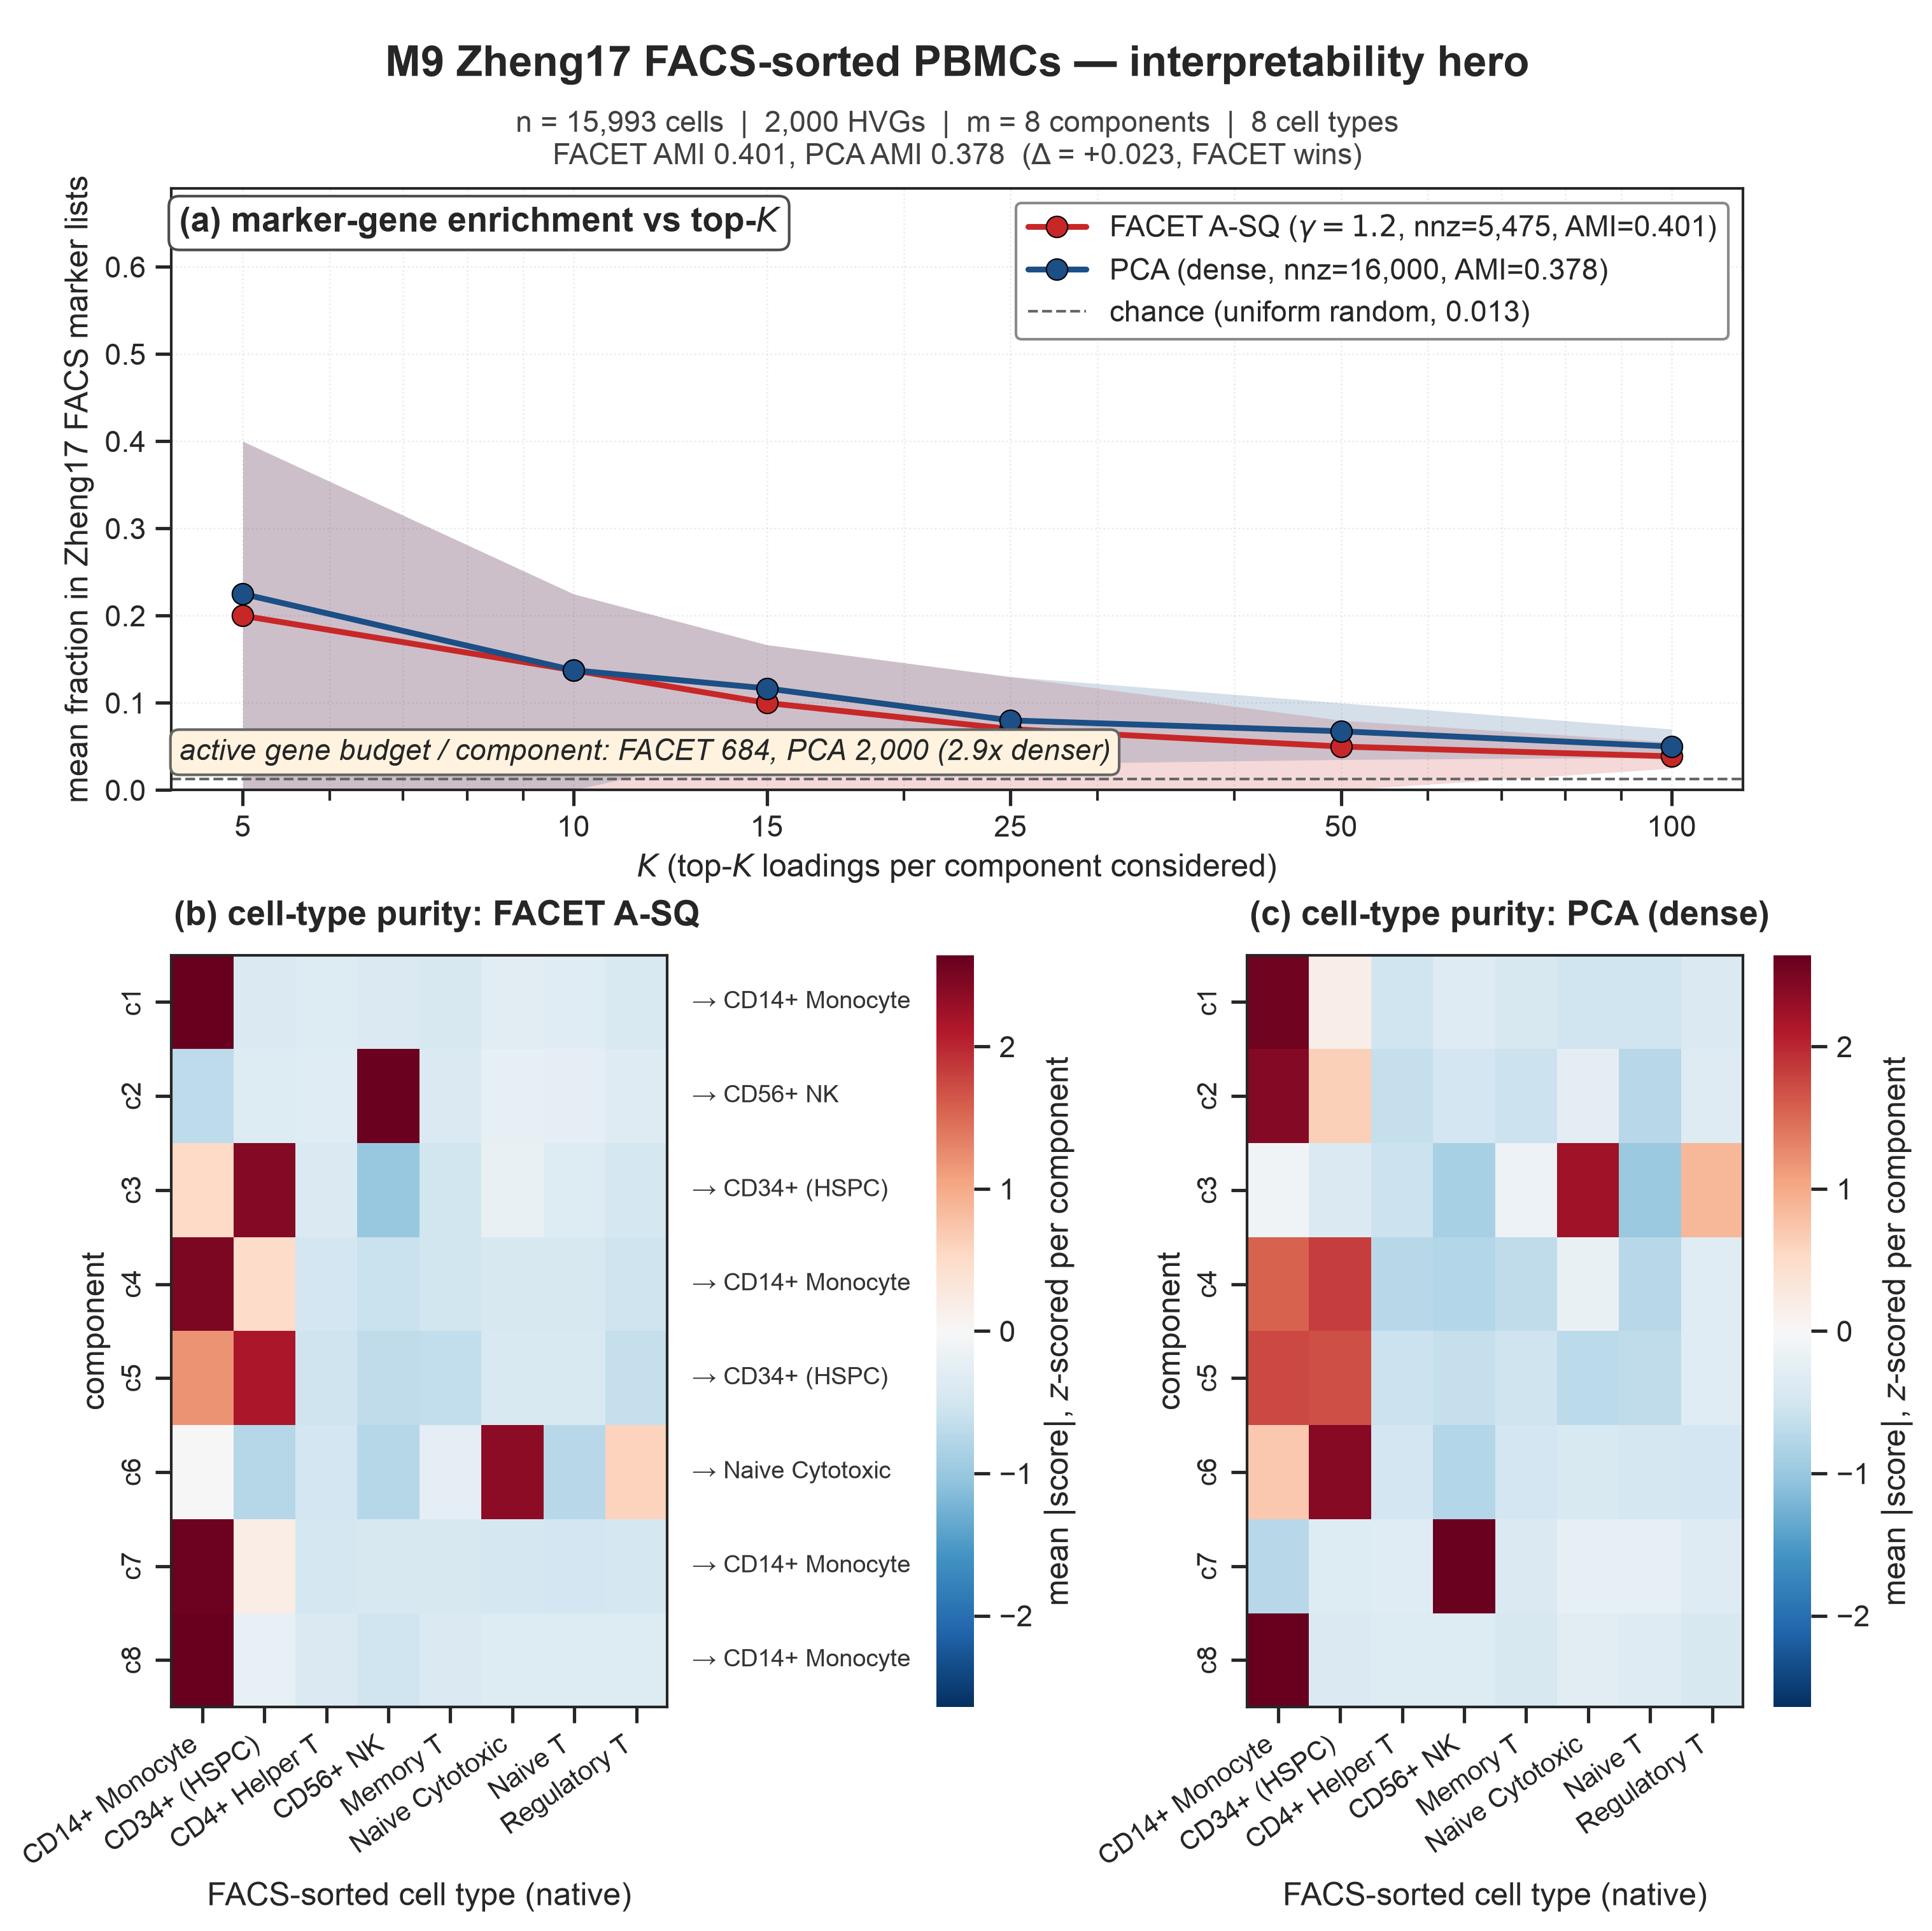
\includegraphics[width=\linewidth]{../shared/figures/generated/m9_zheng_facs_interpretability_hero.png}
 \caption{\textbf{M9 Zheng17 FACS interpretability hero.} Companion to Fig.~\ref{fig:m9-zheng-facs-hero}, interpretability-first panels on the same bead-purified data. \textbf{(a)}~Mean enrichment vs top-$K$ in the Zheng FACS marker list (CD14+ Mono, CD34+, CD4 helper, CD56+ NK, Treg, memory/naive T subsets); gene-economy banner reports the per-component active-gene budget. \textbf{(b)}~FACET cell-type purity heatmap with dominant FACS gate annotated per component (right-hand labels). Each FACET component localises on a single FACS population. \textbf{(c)}~PCA cell-type purity on the same colour scale is visibly more diffuse.}
 \label{fig:m9-zheng-facs-interp}
\end{figure}
